\setcounter{chapter}{14}
\exam{Exame 2015/16}
{
\renewcommand{\thesubsection}{\thesection\alph{subsection}}

\question{Pergunta 1}
\lstinputlisting[language=Python, caption=Programa 2015E-1 (Python3)]{2015E_1.py}
Resposta: \textbf{9.46000}

\question{Pergunta 2}

\question{Pergunta 3}
\lstinputlisting[language=Python, caption=Programa 2015E-3 (Python3)]{2015E_3.py}
\questionitem{Item a}
\begin{center}
    \begin{tabular}{ c c c | c}
        1 & \textbf{0.50000} & \textbf{0.33333} & \textbf{-1.00000} \\
        0 & 1 & \textbf{1.00000} & \textbf{18.00000} \\
        0 & 0 & 1 & \textbf{-30.00000}
    \end{tabular}
\end{center}
\questionitem{Item b}
\begin{equation*}
    \mathbf{x}
    =\begin{bmatrix} x_1 \\ x_2 \\ x_3 \end{bmatrix}
    =\begin{bmatrix} -15.00000 \\ 48.00000 \\ -30.00000 \end{bmatrix}
\end{equation*}
\questionitem{Item c}
\begin{center}
    \begin{tabular}{ c c c | c}
        1 & \textbf{0.50000} & \textbf{0.33333} & \textbf{-0.10000} \\
        0 & 1 & \textbf{1.00000} & \textbf{-0.60000} \\
        0 & 0 & 1 & \textbf{-3.00000}
    \end{tabular}
\end{center}
\begin{equation*}
    \mathbf{x}
    =\begin{bmatrix} x_1 \\ x_2 \\ x_3 \end{bmatrix}
    =\begin{bmatrix} -0.30000 \\ 2.40000 \\ -3.00000 \end{bmatrix}
\end{equation*}
\questionitem{Item d}
A incógnita mais sensível a erros nos dados é $x_3$, dado que possui maior valor absoluto no vetor da estabilidade externa.

}
\question{Pergunta 4}
\questionitem{Item 1}
\lstinputlisting[language=Maxima, caption=Maxima input 2015E-4]{2015E_4.mc}
\begin{center} 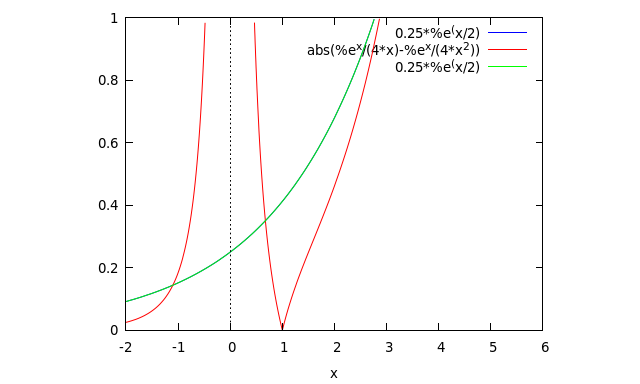
\includegraphics[scale=0.45]{2015E_4} \end{center}
\begin{enumerate}[label=\alph*)]
    \item Converge para as raízes nos intervalos $X_1$ e $X_2$.
    \item Não converge para nenhuma das raízes.
    \item Converge para as raízes nos intervalos $X_1$ e $X_2$.
\end{enumerate}
\questionitem{Item 2}
\lstinputlisting[language=Python, caption=Programa 2015E-4 (Python3)]{2015E_4.py}
\begin{center}
    \begin{tabular}{c | c}
        Iteração & $x$ \\ \hline
        0 & \textbf{1.1000} \\
        1 & \textbf{1.5769}
    \end{tabular}
\end{center}
\questionitem{Item 3}
O resíduo da equação que estou a resolver, ao fim da primeira iteração, é 0.4769.
{
\renewcommand{\thesubsection}{\thesection\alph{subsection}}
\question{Pergunta 5}
\lstinputlisting[language=Maxima, caption=Maxima input 2015E-5]{2015E_5.mc}
\lstinputlisting[language=Python, caption=Programa 2015E-5 (Python3)]{2015E_5.py}
\begin{center}
    \begin{tabular}{l | c c}
        & M. Trapézios & M. Simpson \\ \hline
        $h$ & 0.12500  &       0.12500 \\
        $h'$ & 0.06250  &       0.06250 \\
        $h''$ & 0.03125  &       0.03125 \\
        Comprimento do arco $L_1=I$ & 11.34629 &       11.25550 \\
        Comprimento do arco $L_2=I'$ & 11.27778 &       11.25495 \\
        Comprimento do arco $L_3=I''$ & 11.26063 &       11.25491 \\
        Quociente de convergência $QC$ & 3.99394  &       15.85798 \\
        Erro estimado $\varepsilon$ & 0.00572  &       0.00001
    \end{tabular}
\end{center}
\question{Pergunta 6}
\question{Pergunta 7}
\lstinputlisting[language=Python, caption=Programa 2015E-7 (Python3)]{2015E_7.py}
Resposta: \textbf{2.17500}
}